\documentclass[a4paper,11pt,fleqn,twoside,openright]{memoir} % Brug openright hvis chapters skal starte på højresider; openany, oneside

%%%% PACKAGES %%%%

%  Oversættelse og tegnsætning  %
\usepackage[utf8]{inputenc}					% Gør det muligt at bruge æ, ø og å i sine .tex-filer

\raggedbottom
\usepackage[all]{nowidow}
\usepackage[T1]{fontenc}  % Hjælper med orddeling ved æ, ø og å. Sætter fontene til at være ps-fonte, i stedet for bmp	
\usepackage{syntax} %til BNF
\usepackage{everyshi}
\makeatletter
\let\totalpages\relax
\newcounter{mypage}
\EveryShipout{\stepcounter{mypage}}
\AtEndDocument{\clearpage
   \immediate\write\@auxout{%
    \string\gdef\string\totalpages{\themypage}}}
\makeatother
\usepackage{longtable}
\usepackage{lscape}
\usepackage[lined,boxed,linesnumbered]{algorithm2e}
\usepackage{latexsym}										% LaTeX symboler
\usepackage{xcolor,ragged2e,fix-cm}			% Justering af elementer
\usepackage{pdfpages} % Gør det muligt at inkludere pdf-dokumenter med kommandoen \includepdf[pages={x-y}]{fil.pdf}	
\usepackage{fixltx2e}					% Retter forskellige bugs i LaTeX-kernen
\usepackage{color}
\definecolor{darkgray}{rgb}{0.95,0.95,0.95}
\usepackage{listings}
\usepackage{qtree}
\usepackage{multicol}


 \lstloadlanguages{% Check Dokumentation for further languages ...
         %[Visual]Basic
         %Pascal
         %C
	%[Sharp]C
         %C++
         %XML
         %HTML
         Java
 }
\lstset{ %
inputencoding=utf8,
literate=%
{æ}{{\ae}}1
{å}{{\aa}}1
{ø}{{\o}}1
{Æ}{{\AE}}1
{Å}{{\AA}}1
{Ø}{{\O}}1,
language=Java,                % the language of the code
basicstyle=\footnotesize\ttfamily,       % the size of the fonts that are used for the code
float = H,
xleftmargin = 10pt,
xrightmargin = 10pt,
rulecolor = \color{black},
numbers=left,                   % where to put the line-numbers
numberstyle=\footnotesize,      % the size of the fonts that are used for the line-numbers
stepnumber=1,                   % the step between two line-numbers. If it's 1, each line 
                                % will be numbered
numbersep=5pt,                  % how far the line-numbers are from the code
showspaces=false,               % show spaces adding particular underscores
showstringspaces=false,         % underline spaces within strings
showtabs=false,                 % show tabs within strings adding particular underscores
tabsize=2,                      % sets default tabsize to 2 spaces
captionpos=b,                   % sets the caption-position to bottom
breaklines=true,                % sets automatic line breaking
breakatwhitespace=false,        % sets if automatic breaks should only happen at whitespace
               % show the filename of files included with \lstinputlisting;
                                % also try caption instead of title
escapeinside={\%*}{*)},         % if you want to add a comment within your code
keywordstyle=\color[rgb]{0,0,1},
commentstyle=\color[rgb]{0.133,0.545,0.133},
stringstyle=\color[rgb]{0.627,0.126,0.941},
morekeywords={}
}

% add frame environment
\usepackage[framemethod=TikZ]{mdframed}
\mdfsetup{%
    skipbelow=\topskip,
    skipabove=\topskip,
    leftmargin=50pt,
    rightmargin=0pt,
    backgroundcolor=darkgray,
    middlelinecolor=black,
    roundcorner=10
}

\mdfdefinestyle{RoundStyle}{%
 skipbelow=\topskip,
    skipabove=\topskip,
    leftmargin=0pt,
    rightmargin=0pt,
    backgroundcolor=darkgray,
    middlelinecolor=black,
    roundcorner=10}

% needed for \lstcapt
\def\ifempty#1{\def\temparg{#1}\ifx\temparg\empty}

% make new caption command for listings
\usepackage{caption}
\newcommand{\lstcapt}[2][]{%
    \ifempty{#1}%
        \captionof{lstlisting}{#2}%
    \else%
        \captionof{lstlisting}[#1]{#2}%
    \fi%
    \vspace{0.75\baselineskip}%
}

\usepackage{tabularx}
\usepackage{changepage}

																			
%  Figurer og tabeller floats %
\pdfoptionpdfminorversion=6	% Muliggør inkludering af pdf dokumenter, af version 1.6 og højere
\usepackage{graphicx} 		% Pakke til jpeg/png billeder
\usepackage{rotating}	

%  Matematiske formler og maskinkode 
\usepackage{amsmath,amssymb,stmaryrd} 	% Bedre matematik og ekstra fonte
\usepackage{textcomp}                 	% Adgang til tekstsymboler
\usepackage{mathtools}			% Udvidelse af amsmath-pakken.
\usepackage{siunitx}			% Flot og konsistent præsentation af tal og enheder med \SI{tal}{enhed}

%  Referencer, bibtex og url'er  %
\usepackage{url}	% Til at sætte urler op med. Virker sammen med ref
%\usepackage[danish]{varioref} % Giver flere bedre mulighed for at lave krydshenvisninger
\usepackage[english]{varioref} % Giver flere bedre mulighed for at lave krydshenvisninger
\usepackage{natbib}	% Litteraturliste med forfatter-år og nummerede referencer
\usepackage{xr}		% Referencer til eksternt dokument med \externaldocument{<NAVN>}
\usepackage{nomencl}	% Pakke til at danne nomenklaturliste
\makenomenclature		% Nomenklaturliste

%  Floats  %
\let\newfloat\relax 	% Memoir har allerede defineret denne, men det gør float pakken også
\usepackage{float}
%\usepackage[footnote,draft,danish,silent,nomargin]{fixme}	% Indsæt rettelser og lignende med \fixme{...} Med final i stedet for draft, udløses en error for hver fixme, der ikke er slettet, når rapporten bygges.
\usepackage[final,silent]{fixme}
%\usepackage[draft, danish,silent]{fixme}

%%%% CUSTOM SETTINGS %%%%

%  Marginer  %
\setlrmarginsandblock{3.5cm}{2.5cm}{*}	% \setlrmarginsandblock{Indbinding}{Kant}{Ratio}
\setulmarginsandblock{2.5cm}{3.0cm}{*}	% \setulmarginsandblock{Top}{Bund}{Ratio}
\checkandfixthelayout 

%  Litteraturlisten  %
\bibpunct[,]{[}{]}{;}{a}{,}{,} 	% Definerer de 6 parametre ved Harvard henvisning (bl.a. parantestype og seperatortegn)
\bibliographystyle{bibtex/harvard}	% Udseende af litteraturlisten. Ligner dk-apali - mvh Klein

%  Indholdsfortegnelse  %
\setsecnumdepth{subsubsection}	% Dybden af nummerede overkrifter (part/chapter/section/subsection)
\maxsecnumdepth{subsubsection}	% Ændring af dokumentklassens grænse for nummereringsdybde
\settocdepth{section} 		% Dybden af indholdsfortegnelsen


%  Visuelle referencer  %
\usepackage[colorlinks, bookmarksnumbered, bookmarksdepth=4]{hyperref} % Giver mulighed for at ens referencer bliver til klikbare hyperlinks. .. [colorlinks]{..}
%\usepackage{memhfixc}
\hypersetup{pdfborder = 0 0 0}	% Fjerner ramme omkring links i fx indholsfotegnelsen og ved kildehenvisninger 
\hypersetup{			%	Opsætning af farvede hyperlinks
    colorlinks = false,
    linkcolor = black,
    anchorcolor = black,
    citecolor = black
}
\usepackage{footnote}
\makesavenoteenv{tikzpicture}

\definecolor{gray}{gray}{0.80}					% Definerer farven grå

%  Kapiteludssende  %
\definecolor{numbercolor}{gray}{0.7}			% Definerer en farve til brug til kapiteludseende
\newif\ifchapternonum

\makechapterstyle{jenor}{			% Definerer kapiteludseende -->
  \renewcommand\printchaptername{}
  \renewcommand\printchapternum{}
  \renewcommand\printchapternonum{\chapternonumtrue}
  \renewcommand\chaptitlefont{\fontfamily{pbk}\fontseries{db}\fontshape{n}\fontsize{25}{35}\selectfont\raggedleft}
  \renewcommand\chapnumfont{\fontfamily{pbk}\fontseries{m}\fontshape{n}\fontsize{1in}{0in}\selectfont\color{numbercolor}}
  \renewcommand\printchaptertitle[1]{%
    \noindent
    \ifchapternonum
    \begin{tabularx}{\textwidth}{X}
    {\let\\\newline\chaptitlefont ##1\par} 
    \end{tabularx}
    \par\vskip-2.5mm\hrule
    \else
    \begin{tabularx}{\textwidth}{Xl}
    {\parbox[b]{\linewidth}{\chaptitlefont ##1}} & \raisebox{-15pt}{\chapnumfont \thechapter}
    \end{tabularx}
    \par\vskip2mm\hrule
    \fi
  }
}			% <--

\chapterstyle{jenor}	% Valg af kapiteludseende - dette kan udskiftes efter ønske
\usepackage{wrapfig}


%\renewcommand{\headrulewidth}{0.4pt}
%\renewcommand{\footrulewidth}{0.4pt}

\usepackage{enumitem}
% Sidehoved %

\makepagestyle{custom} % Definerer sidehoved og sidefod - kan modificeres efter ønske -->
\makepsmarks{custom}{																						
\def\chaptermark##1{\markboth{\itshape\thechapter. ##1}{}} % Henter kapitlet den pågældende side hører under med kommandoen \leftmark. \itshape gør teksten kursiv
\def\sectionmark##1{\markright{\thesection. ##1}{}}	% Henter afsnittet den pågældende side hører under med kommandoen \rightmark
} % Sidetallet skrives med kommandoen \thepage	
\makeevenhead{custom}{\leftmark}{}{Group SW615F14} % Definerer lige siders sidehoved efter modellen \makeevenhead{Navn}{Venstre}{Center}{Højre}
\makeoddhead{custom}{Group SW615F14}{}{\leftmark} % Definerer ulige siders sidehoved efter modellen \makeoddhead{Navn}{Venstre}{Center}{Højre}

\usepackage{lastpage}
\usepackage{ifthen}
\usepackage{intcalc}
\usepackage{nth}

\makeevenfoot{custom}{Page \thepage}{}{Aalborg University}	% Definerer lige siders sidefod efter modellen \makeevenfoot{Navn}{Venstre}{Center}{Højre}
\makeoddfoot{custom}{Aalborg University}{}{Page \thepage}% Definerer ulige siders sidefod efter modellen \makeoddfoot{Navn}{Venstre}{Center}{Højre}		
\makeheadrule{custom}{\textwidth}{0.5pt}	 % Tilføjer en streg under sidehovedets indhold
\makefootrule{custom}{\textwidth}{0.5pt}{1mm}	% Tilføjer en streg under sidefodens indhold

\copypagestyle{nychapter}{custom} % Følgende linier sørger for, at sidefoden bibeholdes på kapitlets første side
\makeoddhead{nychapter}{Group SW615F14}{}{\leftmark}
\makeevenhead{nychapter}{Group SW615F14}{}{\leftmark}
\makeheadrule{nychapter}{\textwidth}{0pt}
\aliaspagestyle{chapter}{nychapter}	% <--
\aliaspagestyle{cleared}{custom}

\pagestyle{custom}

\usepackage{newfloat}

%%%% CUSTOM COMMANDS %%%%

\let\originaltable\table
\let\endoriginaltable\endtable
\renewenvironment{table}[1][h!t]{%
  \originaltable[#1]
  \centering}%
  {\endoriginaltable}

% Billede hack %
\newcommand{\figur}[4]{
		\begin{figure}[H] \centering
			\includegraphics[width=#1\textwidth]{billeder/#2}
			\caption{#3}\label{#4}
		\end{figure} 
}

% højrepil %
\newcommand{\ra}[0]{\rightarrow}
% epsilon %
\newcommand{\eps}{\varepsilon}

%navne macro
\usepackage{xspace}
\newcommand{\piko}{\textit{Piktooplæser}\xspace}
\newcommand{\ol}{\textit{Oasis Library}\xspace}
\newcommand{\oa}{\textit{Oasis App}\xspace}
\newcommand{\ps}{\textit{Pictosearch}\xspace}
\newcommand{\ldb}{\textit{LocalDB}\xspace}
\newcommand{\pa}{\textit{Parrot}\xspace}
\newcommand{\pt}{\textit{Piktotegner}\xspace}
\newcommand{\cat}{\textit{Kategoriværktøjet}\xspace}

% Vektor hack %
\newcommand{\vektor}[3]{
			$\begin{pmatrix}
				#1 \\ #2 \\ #3
			\end{pmatrix}$
}

% declare the floating environment {Grammar}
% this will also define \listofGrammars:
\DeclareFloatingEnvironment[
  % the file extension for the file used to create the list:
  fileext   = logr,% don't use log here!
  % the heading for the list:
  listname  = {List of Grammars},
  % the name used in captions:
  name      = Grammar,
  % the default floating parameters if the environment is used
  % without optional argument:
  placement = H
]{Grammar}

%grammatik
\newenvironment{grammatik}[2]
{
\def\fooNoI{#1} \def\fooNoII{#2}
\begin{Grammar}
\begin{grammar}
}
{
\end{grammar}
\caption{\fooNoII}\label{gra:\fooNoI}
\end{Grammar}
}

%tikz
\usepackage{tikz}
\usetikzlibrary{positioning}
\usetikzlibrary{shadows}
\usetikzlibrary{shapes,arrows}
\tikzstyle{mynodestyle} = [draw,outer sep=3,inner sep=3,minimum size=10,line width=1, very thick, draw=black!55, top color=white,bottom color=black!20]

\usetikzlibrary{arrows}
\tikzstyle{io} = [font={\bfseries},trapezium,trapezium left angle=70,trapezium right angle=-70,minimum height=0.5cm,line width=1, text=black, very thick, draw=black!55, top color=white, align=center ]
\tikzstyle{linear} = [draw, -latex']
\tikzstyle{cirkel} = [ font={\bfseries}, shape=circle, outer sep=4,minimum size=0.5cm, text=black, very thick, draw=black!55, top color=white, align=center]
\tikzstyle{cirkelgray} = [ font={\bfseries}, shape=circle, outer sep=4,minimum size=0.5cm, text=black, very thick, draw=black!55, top color=gray, align=center]
\tikzstyle{firkant} = [ font={\bfseries},outer sep=4,inner sep=7,minimum size=0.5cm,line width=1, text=black, very thick, draw=black!55, top color=white, align=center]
\tikzstyle{firkantgray} = [ font={\bfseries},outer sep=4,inner sep=7,minimum size=0.5cm,line width=1, text=black, very thick, draw=black!55, top color=gray, align=center]
\tikzstyle{tekst} = []
\tikzstyle{bendH} = [bend right=40, -triangle 60, color=red]
\tikzstyle{bendV} = [bend left=40, -triangle 60, color=red]
\tikzstyle{afrundetFirkant} = [ rounded corners ,font={\bfseries},outer sep=4,inner sep=7,minimum size=0.5cm,line width=1, text=black, very thick, draw=black!55, top color=white, align=center]
\tikzstyle{rude} = [ draw, diamond, aspect=2 ,font={\bfseries},outer sep=4,inner sep=7,minimum size=0.5cm,line width=1, text=black, very thick, draw=black!55, top color=white, align=center]
\tikzstyle{sortCirkel} = [cirkel, black, top color=black, bottom color = black]
\tikzstyle{sortCirkelPrikInner} = [cirkel, white, top color=black, bottom color = black, minimum size=0.5cm]
\tikzstyle{sortCirkelPrikOuter} = [cirkel, black, top color=white, bottom color = white, minimum size=0.7cm]
\tikzstyle{DB} = [draw=black,cylinder,shape border rotate=90,shape aspect=.25,font={\bfseries}]

%kode
\newcommand{\kode}[3]{
\noindent
\newline
\newline
\begin{minipage}{\textwidth}
\begin{mdframed}
		\lstinputlisting{kode/#3}

\end{mdframed}\lstcapt{#1}\label{lst:#2}
\end{minipage}
}

\newenvironment{code}[2]
{\def\fooNoI{#1} \def\fooNoII{#2}\noindent\newline \begin{minipage}{\textwidth}\begin{mdframed}[style=RoundStyle]}{\end{mdframed}\lstcapt{\fooNoII}\label{\fooNoI}\end{minipage}}

% quotering
\newcommand{\gaas}[{1}]{``#1''}

% lilleitem
%\newenvironment{noindlist}
 %{\vspace{-5mm}\begin{list}{\labelitemi}{\leftmargin=1em \itemindent=0em }
%\addtolength{\itemsep}{-0.5\baselineskip}}
 %{\end{list}
%\vspace{-20em}}

\newcommand{\Tau}{\mathrm{T}}

\newlist{Description}{description}{1}
\setlist[Description]{labelindent=2\parindent,leftmargin=2\parindent}

\newenvironment{inddes}
 {\begin{description}[font=$\bullet$\scshape\bfseries, labelindent=2\parindent,leftmargin=2\parindent]
 }
 {\end{description}}

\newenvironment{noindlist}
 {\vspace{-5mm}\begin{list}{\labelitemi}{\leftmargin=1em \itemindent=0em }
        \setlength{\topsep}{0pt}
        \setlength{\parskip}{0pt}
        \setlength{\partopsep}{0pt}
        \setlength{\parsep}{0pt}         
        \setlength{\itemsep}{0pt} }
 {\end{list}}

\newcommand{\doublesignaturestart}[2]{%
  \parbox{\textwidth}{
    \centering Aalborg, \today\\
    \vspace{2cm}

    \parbox{7cm}{
      \centering
      \rule{6cm}{1pt}\\
       #1 
    }
    \hfill
    \parbox{7cm}{
      \centering
      \rule{6cm}{1pt}\\
      #2
    }
  }
}

\newcommand{\longtablesetting}[1]{
\endhead
\multicolumn{#1}{c}{\textit{Continued on next page}} \\
\endfoot
\endlastfoot
}

\newcommand{\subsubsubsection}[1]{
\noindent
\textbf{#1}
}

\newcommand{\doublesignature}[2]{%
  \parbox{\textwidth}{
\vspace{2cm}
    \parbox{7cm}{
      \centering
      \rule{6cm}{1pt}\\
       #1 
    }
    \hfill
    \parbox{7cm}{
      \centering
      \rule{6cm}{1pt}\\
      #2
    }
  }
}

\newcommand{\strips}[3]{
\noindent \textbf{#1}\\
\indent \textbf{Precond:} #2\\
\indent \textbf{Effect:} #3\\\newline
}

%%%% ORDDELING %%%%

\hyphenation{hvad hvem hvor listOfErrors}
\newcolumntype{R}{>{\raggedright\arraybackslash}X}

%----------------SPROG------------------------
%----------------dk
%\usepackage[danish]{babel}							% Dansk sporg, f.eks. tabel, figur og kapitel
%\renewcommand{\algorithmcfname}{Algoritme}
%\renewcommand*{\lstlistingname}{Kodeudsnit}
%----------------en
\usepackage[english]{babel}
\usepackage{cleveref}


\usepackage{pdflscape}




%%% TO DO %%%
\usepackage[colorinlistoftodos]{todonotes}

\newcommand{\namedtodo}[5]
{
  \ifthenelse{\equal{#1}{}}
  {
    \todo[backgroundcolor=#4,caption=
    {\textbf{#3: } #2}
    ,inline]
    {\color{#5}\textbf{#3: }#2}
  }
  {
    \todo[backgroundcolor=#4,caption=
    {\textbf{#3: } #1}
    ,inline]
    {\color{#5}\textbf{#3: }#2}
  }
}
\newcommand{\Alexander}[2][]{\namedtodo{#1}{#2}{Alexander}{green}{black}}
\newcommand{\Christoffer}[2][]{\namedtodo{#1}{#2}{Christoffer}{orange}{black}}
\newcommand{\Dan}[2][]{\namedtodo{#1}{#2}{Dan}{blue!80}{white}}
\newcommand{\Kristian}[2][]{\namedtodo{#1}{#2}{Kristian}{black!10!yellow!90}{black}}
\newcommand{\Ivan}[2][]{\namedtodo{#1}{#2}{Ivan}{black!10!red!90}{white}}


  \makeatletter \renewcommand \listoftodos{\section*{List of Todos} \@starttoc{tdo}}
  \renewcommand\l@todo[2]
    {\par\noindent \textit{#2}, \parbox{10cm}{#1}\par} \makeatother

\begin{document}

% Forindhold - nummereres med romertal
\frontmatter 
\thispagestyle{empty}
\begin{flushright}
\vspace{3cm}

\phantom{hul}

\phantom{hul}

\phantom{hul}

\textsl{P8 Project} \\ \vspace{1cm}

\rule{1\textwidth}{3mm} \\ \vspace{1.5cm}
%\vspace{1cm}

\includegraphics[width=\textwidth]{Images/frontpage.jpg}
\vspace{1.5cm} \\
\textsc{\Large Tempo Player - The music player that fits YOUR tempo \\ \Ivan{Metaphor - Think about more suitable title.}
P8 Project\\
Group SW802F15\\
Software\\
Department of Computer Science\\
Aalborg University\\
Spring 2015\\
~\\
}

\end{flushright}

\cleardoublepage
\begin{nopagebreak}
	{\samepage 
		\begin{tabular}{r}
			\parbox{16cm}
			{\raisebox{11mm}
				{
\includegraphics[height=3.5cm]{Content/TitlePage/aauIcon.png}}
				\hfill \parbox{8.5cm}{\vspace{-5cm}
				\begin{tabular}{l}
					{\small \textbf{Department of Computer Science}}\\
					{\small Selma Lagerløfs Vej 300} \\
					{\small 9220 Aalborg Ø} \\
					{\small Phone (+45) 9940 9940} \\
					{\small Fax (+45) 9940 9798} \\
					{\small \url{http://www.cs.aau.dk}}
				\end{tabular}}
			}
		\end{tabular}
		
		\begin{tabular}{cc}
			\parbox{7cm}{
				\begin{description}
					\item {\textbf{Title:}} \\
						Intelligent Music with Peer-To-Peer Sharing\\
					
					\item {\textbf{Subject:}} \\
						Mobile Systems\\	
						
					\item {\textbf{Project period:}}\\
						  02-02-2015 -- 27-05-2015\\

					\item {\textbf{Project group:}}\\
						  SW802F15\\
			
					\item {\textbf{Participants:}}\\
						Alexander Drægert\\
						Christoffer\\
						Dan\\
						Kristian Thomsen \\
						  
					\item {\textbf{Supervisor:}}\\
						Ivan Aaen\\
			
					\item {\textbf{Printings:} ? }
					
					\item { \textbf{Pages:} ?? }
					 
					\item { \textbf{Appendices:} ? }
					
					\item { \textbf{Total pages:} ?? }
					
					\item { \textbf{Source code:}\\ 
					{\small \mbox{\footnotesize\url{https://github.com/SW802F15/SourceCode/tree/???????}}}}
			
				\end{description}
				\vfill 
			}
			&	 
			\parbox{6cm}{
				\hfill \\ \\
				\begin{tabular}{l}
					{Abstract:\smallskip}\\ 
					\fbox{
						\parbox{6cm}{
							\bigskip{
								\vfill
								{\small 
									This report contains
Lorem ipsum dolor sit amet, consectetur adipiscing elit. Cras consectetur tristique justo, vel pellentesque augue porttitor ut. Suspendisse potenti. Aliquam ipsum metus, commodo eget eros eu, consectetur auctor turpis. Suspendisse potenti. Sed ut felis elit. Proin eget urna placerat ante rutrum scelerisque ac id neque. Quisque gravida porttitor pulvinar. Fusce feugiat arcu at quam hendrerit, nec ultrices dui fermentum. Nam non nibh ac ligula suscipit dictum. Ut sit amet massa at massa ornare lobortis et ac neque. Duis vulputate mauris sit amet dictum iaculis. Praesent tellus velit, lobortis ac elit in, laoreet efficitur tortor. Etiam blandit, mi ac tincidunt tincidunt, ante sapien efficitur leo, eu efficitur nisi elit condimentum sem. Mauris vulputate neque ut lorem consequat semper. Praesent non tempus tellus.
									\smallskip
								}
							}
						}
					}
				\end{tabular}
			}
		\end{tabular}
		\\ \\
	}
\noindent{\footnotesize\emph{The content of the report is freely available, but may only be published (with source reference) with consent from the authors.}}
\end{nopagebreak}
\cleardoublepage
\chapter{Preface}


















~\\\\
\doublesignaturestart{Alexander Drægert}{Christoffer N'Dûru}
\doublesignature{Dan Petersen}{Kristian Thomsen}
\cleardoublepage

% Indholdsfortegnelse (TOC)
\setlength\parskip{0ex} % Fjerner den vertikale afstand mellem hver linie i indholdsfortegnelse
\tableofcontents* % Indholdsfortegnelsen 
\setlength{\parskip}{3mm} % Aktiverer afstanden igen for resten af rapporten (afstem med preamble!)
%\addtocontents{toc}{\protect\newpage} % Fremtvinger sideskift i indholdsfortegnelsen hvis nødvendig


 % Hovedindhold - nummereres fra side 1
\mainmatter
\makeevenfoot{custom}{Page \thepage~of \pageref{LastPage}}{}{Aalborg University} % Definerer lige siders sidefod efter modellen \makeevenfoot{Navn}{Venstre}{Center}{Højre}
\makeoddfoot{custom}{Aalborg University}{}{Page \thepage~of \pageref{LastPage}} % Definerer ulige siders sidefod efter modellen \makeoddfoot{Navn}{Venstre}{Center}{Højre}		
\pagestyle{custom}

% Rapportindhold
\chapter{Introduction}
\label{chap:intro}
%First Problem - Idea Domain%
Running is a popular form of exercise, however, it can be a tedious and uninspiring endeavour.
To improve the experience, \citet{musicRunEffectArticle} found that 
\textit{``... participants enjoyed what they were doing [running] more when they were listening to music of any sort when compared to when they were not.''}

It was further concluded by \citet{musicRunEffectArticle} that the volume and tempo of the music influenced the running experience.
They concluded that the running pace for novice runners, while listening to relatively low-tempo music, was slower than when not listening to music. Additionally listening to high-tempo music resulted in a faster running pace, compared to when not listening to music.

This conclusion is in disagreement with the conclusion of \citet{musicNoPerformanceEffect} which suggests, that \textit{``... music had no impact on mean power output.''}. \citet{musicNoPerformanceEffect} measure the running pace by mean power output, nevertheless, they did not see any impact on the running pace by listening to music.

As a result, we can not definitively conclude whether music of different tempo will affect the running experience differently. 
However by adhering to \citet{musicRunEffectArticle}'s conclusion, we can only improve the running experience, since \citet{musicNoPerformanceEffect} concludes there can be no negative impact, by playing music.

Today many runners use their smartphone as a music player, which can either be placed in their hand, pocket, or on their arm.
The sensors in a smartphone enable monitoring the pace and speed of the runner.
Based on this knowledge the first problem can be stated:

\begin{center}
\textit{How can we provide music with an appropriate tempo, compared to the current pace, to the runner through the use of a smartphone?}
\end{center}

%Second Problem - UI%
\noindent Operating a smartphone while running is difficult, especially if it is placed in the pocket or on the arm of the runner.
In order for the runner to operate the smartphone; play, pause, stop, or change song, the runner would have to stop running, or focus more than normally. This can disrupt the runner's form, and lead to injuries and accidents.
Based on this knowledge the second problem can be stated: 

\begin{center}
\textit{How can a smartphone application be operated without disrupting the runner's form and/or concentration?}
\end{center}
%Third Problem - Methodology%
%\noindent Most large scale software projects fail. 
\noindent According to \citet{gartner:failure} \textit{``A full 66 percent of large scale projects fail ...”}, and although this is not a large scale project, some of the same pitfalls exist.
One way to avoid some of these pitfalls, is \textit{``... using a structured systems development methodology ...”}, since it according to \citet{dorsey:methodologyReason} \textit{``... is one of the critical success factors in a systems development project.”}.

We will in this project focus on the development methodology \texttt{Extreme Programming} (XP).
XP is used because its an interesting methodology and it is development oriented.
Furthermore, XP's requirements of self-organising teams, iteration length, and team size fit well with this project. 
Based on this knowledge the third problem can be stated:

\begin{center}
	\textit{How do we adapt the structured systems development methodology, Extreme Programming, to our project?}
\end{center}

\chapter{Analysis}
\label{chap:analysis}
\section{Problem Domain}
\section{Problem Statement}
Running is a popular form of exercise, however it can be a tedious and uninspiring endeavour.
To improve the experience, \citet{musicRunEffectArticle} found that 
\textit{``... participants enjoyed what they were doing [running] more when they were listening to music of any sort when compared to when they were not.''}

It was further discovered by \citet{musicRunEffectArticle} that the volume and tempo of the music influenced the running experience.
They discovered that the running speed, while listening to relatively slow music, was slower than when not listening to music. Additionally listening to fast-paced music resulted in a faster running speed, compared to when not listening to music.

Today many runners use their smartphone as a music player, which can either be placed on their arm or in their pocket.
The sensors in a smartphone allows for reading the steps per minute and speed of the runner.

\begin{center}
\textit{How can this data be used and calculated upon to provide the runner with an enjoyable running experience?}
\end{center}

\Ivan{Will the app follow the users tempo or will the user follow the music?}
\Ivan{Think about and discuss difference types of running e.g. interval.}
\Ivan{Maybe have options to choose between 3 mode: plain (music follows user), fast (user follows music), interval or other template (user follows music of different BPM).}

With a smartphone placed on their arm or in their pocket, it is difficult to navigate applications through visual feedback. Furthermore operating the smartphone while running decreases the navigability of the smartphone. \Alexander{SOURCE} 
The runner's form should not be disrupted by navigating. 
\Alexander{Re-write last (previous $\uparrow$) line.}

\begin{center}
\textit{How can a smartphone application be operated without disrupting the runner's form?}
\end{center}


\chapter{Methodology}
\label{chap:methodology}
\section{What is eXtreme Programming?}
What is the XP methodology?
What does Extreme mean? E.g. Review is much more important and useful, so turn it up in comparison to other methodologies.
Start of Beck books.
\section{Extreme Programming versus Scrum}
\Ivan{motiver sammanligningen}
\Alexander{Write something about Scrum being the most (by far) known and used agile methodology, hence a comparison is warranted.}
\Kristian{why do we even have this section?, from mountaingoatsoftware}
The two are similar, both being agile methodologies with self-organising teams, however there exists some significant differences.

The most significant difference, is that Scrum does not have any development oriented practises.
XP on the other hand, has plenty of development oriented practises. Practises such as pair programming, test-driven development, refactoring, automated testing, simple design, and so forth.

Another difference is the flexibility of the iteration, or sprints as they are called in Scrum.
When a sprint is planned and started, the sprint backlog is not susceptible to change.
The iteration backlog in XP can be changed, as long as the swapped features are not in progress.

The last significant difference is the role responsible for prioritising the work order.
In Scrum the Product Owner prioritises the product backlog, but the developers choose the work order.
In XP the customer prioritises the product backlog, and the developers must work following this prioritisation. 

\Ivan{evt. diskuter forskellenes betydning for jer}
\Alexander{If we have time, it would be a nice suggestion, but at this time it is not likely.}
\section{eXtreme Programming as applied in this project}
What is the priciples of XP.
What is the formål of XP.
How do we expect it to be used?

\Alexander{When to use task, story, task card, story card, user story, use case?}
\Alexander{When to use solution, program, project, product?}
\section{Adaptation of Extreme Programming}
This project is developed with an educational purpose, to which some requirements and restrictions exist.
Partly due to these requirements and restrictions, we made some adaptations to XP for it to fit inside the project parameters.

\subsection{40-hour Week}
The purpose of this practise is to ensure energetic developers every day, and not to overwork them to the point of burnout as explained by \citet[p. 58]{xp:explored}.
We will implement this practise by timeboxing the project time.
This way we will still be able to ensure rested and energetic developers, regardless of courses and other non-project matters.

%While we are working on this project, we also follow a range of courses as part of our education.
%As a result of this, our schedule will be fragmented when counting project time, as opposed to a real world contract, were the schedule would be non-fragmented.
%We will therefore not be able to use the literal implementation of this practise.

\subsection{Code Standards}
Creating a formal code standard is a time consuming task.
We expect that creating a formal code standard, when we already have an informal code standard, will be too time consuming compared to the benefits.
The informal code standard has been created and expanded through our previous experiences of working together.

\subsection{Collective Ownership}
As explained by \citet[p. 54]{xp:explored}, this practise supports flexible and quick changes, however some risks still exist.
The problems most likely to occur in this project are: lack of expertise, violating private space, and personal pride.

The problem with lack of expertise occurs when a problem is just passed on, without anyone having any expertise in the overall problem.
By using Pair Programming the expertise will be spread to the entire team, ensuring everyone obtains knowledge about the overall problems.

The problem of violating each others' private space, refers to when developers need to access and work in the same document. This can cause developers to stay at their current version and only code there, in order to avoid conflicting documents.
However, by using Continuous Integration it will be impossible to be stuck on an old version.
By using the Testing practise, it is ensures changes will not compromise the existing code.

The problem with personal pride is not directly addressed by XP.
This problem can occur if a developer becomes proud of their work, and does not want to see it ``ruined'' by others.
This is a problem we will have to watch out for and to remind ourselves of XP's saying: ``Be brave''.
 

\subsection{Continuous Integration}
According to \citet[p. 57]{xp:explored} this practise should be automated through the setup of a dedicated build server.
Making this an automated task, should ensure the developers working on the current version.
The integration itself should not be automated, but the build and testing should, i.e., when a story is completed, the changes are integrated into the current build.
The build server then automatically builds and tests the build.
If the tests are not at a 100\%, the developers must fix their code or discard it, to ensure the build always passes 100\% of the tests.

Even though finding and setting up a build server would be the correct way of doing things, we will manually integrate and build the code from a dedicated branch.
We will do this because, we believe we can achieve the same benefits with the manual approach, without using time to set up the build server.
This is only viable because of the small size of the project, which results in short build times and a limited risk of fragmented versions.

\subsection{Metaphor}
The metaphor is an effective way to get a shared vision for the project.
A meaningful metaphor helps create and name the correct objects and actions as described by \citet[p. 87]{xp:explored}.

We see this project as a music player that plays music with a tempo matching the user's pace.
This metaphor might change throughout this project.

\subsection{On-site Customer}
Since this is a semester project, we will not have an actual customer.
In place of the on-site customer, we will act as a surrogate customer.
This means that we are responsible for the priority, requirement decisions, and creation of acceptance tests, as well as other tasks normally done by the customer.

\subsection{Pair Programming}
To fully utilise pair programming, we will borrow two sets of monitors, keyboards, and mice.
We will connect these to our laptops to create two workstations ready for pair programming.

There exists several versions of how to program in pairs. We will try different methods to experience the advantages, and disadvantages of the different versions.

\subsection{Planning Game}
Planning is important. It lets you know how fast you work, what to do next, provides an effective means of communication with the customer, and allows you to quickly respond to changes \citet[p. \Kristian{Find page number}]{xp:explored}. 
\Kristian{grep for bad cites?}

In XP planning happens in two stages. There is the release planning and the iteration planning.
The release planning event, as explained by \citet[p. \Kristian{Find page number}]{xp:explored}, is where the customer writes all the user stories, he wants the program to cover.
The developers then estimate the time it will take to implement the different stories.
Then the customer prioritises the stories by what should be done first.
Finally the stories to be done in the release are selected based on project velocity, and priority of each story.

The iteration planning event, as explained by \citet[p. \Kristian{Find page number}]{xp:explored}, is where the customer selects which of the stories, from the release plan, he wants implemented in the upcoming iteration.
Usually the highest prioritised stories are chosen, but often these are superseded by the stories not completely implemented last iteration.
The customer is asked to choose a number of stories, based on the project velocity, so the developers are not overworked.

A story can be estimated individually, or collaboratively. Both methods have strengths and weaknesses.
We decided to collaboratively estimate stories, as that approach allows us to use our combined experience to find the right estimation.

\subsection{Refactoring}
As mentioned by \citet[p. \Kristian{Find page number}]{xp:explored}, XP prescribes refactoring to be done on the spot when a bad smell is identified, to prevent building on top of bad code.
Although refactoring is important, we will evaluate each bad smell by severity and time needed to fix, before correcting it.
We will then decide if it is worthwhile to correct the bad smell, compared to implementing new features. Otherwise it will be created as a task/story.

\subsection{Simple Design}
To implement a simple design, we will structure our code in modules.
Each module will contain multiple classes, which all will be short and readable.
To improve readability we will name methods after their function and only implement features with an immediate purpose. This will prevent having code that is never used.

\subsection{Small Releases}
The purpose of this practise is to reduce the risks if changes in the use domain occur, as explained by \citet[p. \Kristian{Find page number}]{xp:explored}.
Although releases are frequent, they must only contain complete features.

This project contains three major features, which we will try to match to approximately three releases.
With each release we will have a complete feature, which then will be user tested and the feedback will be implemented in the next release.

\subsection{Testing}
Testing covers both unit testing and acceptance testing, both are important parts of XP.

Unit tests are created to ease the refactoring process, by ensuring the external behaviour has not been compromised after a change has been made.
We will, as recommended by XP, make use of Test-Driven Development (TDD).

Acceptance tests are created to ensure the product satisfies the customers needs.
Acceptance tests are written by the customer, which we will do ourselves, seeing as we use ourselves as a surrogate customer.

\chapter{Step Counter}
\label{chap:stepCounter}
In the following sections, the development of our step counter module will be explained.
\Christoffer{Intro omskrives?}
\section{User Stories}
\subsection{Step Counter}
\story{Detect the pace of the user.}{High}
{As a user, I, want the application to detect my pace and display it on the screen. }
{\begin{itemize}
\item When I run the screen displays my SPM.
\end{itemize}}

\story{Select song based on pace.}{High}
{As a user, I, want the application to select song to play based on my pace.}
{\begin{itemize}
\item When I run the application automatically selects songs matching my pace.
\end{itemize}}
\section{Specification}

\section{Implementation}
The Step counter is implemented as a single class extending the \texttt{Service} class in Android. The service is started and bound from the \texttt{MusicPlayerActivity}, meaning in our implementation it is launched and closed together with the \texttt{MusicPlayerActivity}. On its creation the \texttt{StepCounterService} registers the accelerometer sensor in order to read data required for step detection.


\subsection{Step Detection}\label{sec:stepCnt}
To determine whether a step is taken, the approach taken by \citet{zhao:pedometer} is implemented. Our implementation first calculates a threshold, which corresponds to the threshold line in \Cref{fig:zhaoGraph}. The threshold is calculated by subtracting the minimum accelerometer measurement from maximum measurement, from the array where the measurements are stored.

According to \citet[p. 2]{zhao:pedometer} a step has occurred if there is a negative slope in the acceleration graph and the acceleration curve crosses the threshold. It is determined whether a negative slope has occurred, by comparing the latest accelerometer measurement with the previous one. If the last measurement was above the threshold, and the current is below the threshold, a negative slope which crossed the threshold and thus, a step has occurred.

As \citet[p. 2]{zhao:pedometer} we assume that a person can either run as fast as five steps per second or walk as slowly as one step every two seconds. This is handled in the implementation by checking the time since the last measurement. If less than 200 milliseconds have passed since the last step, a new step is not detected. If more than 2 seconds have passed the SPM array is updated with a 0 to indicate that the person is not moving (0 steps per minute).

Our implementation utilises an sensitivity limit so measurements which are very close to each other are not detected as a new step, even though they fulfill the requirements mentioned earlier. This is done to filter out small deviations in measurements which might falsely be identified as a new step. The current limit value is 2, and was found experimentally.
\begin{figure}[h!]
  \centering
    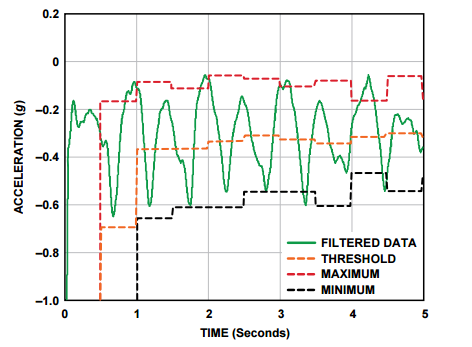
\includegraphics[scale=0.8]{Images/accPlot.png}
  \caption{An acceleration plot from \citet[p. 2]{zhao:pedometer} showing filtered data from a pedometer worn by a person walking.}
  \label{fig:zhaoGraph}
\end{figure}


\subsection{Calculation of Steps Per Minute}
The gab between steps are used to calculate the number of steps the user takes per minute (SPM).

First, the amplitude is calculated which represents the change x, y, z values obtained from the accelerometer. The formula used for this is $$amplitude = \sqrt{x^{2} + y^{2} + z^{2}}$$

The array containing accelerometer measurement data is then updated with the newly calculated value. The data in this array is used for determining whether a step is taken or not, the implementation of which is described in \Cref{sec:stepCnt}.

If we detect a step we look when the previous step was taken and calculate SPM from that, this value is then stored in the array containing the SPM measurements. Afterwards, the average value of the SPM array with the new value is calculated, and the GUI is updated with a new value through a GUI manager.

If no step is taken and more than 2 seconds have passed, the implementation interprets this as if no steps are being taken and the SPM array and GUI is updated with the value 0.

\chapter{Reflection of Methodology}
\label{chap:reflectionMethodology}
\section{Reflection of eXtreme Programming practices}

\paragraph{Example - Pair Programming} was first used to implement all methods. We found this to be inefficient in cases where there were the need for a lot of research or the implementation was trivial.


\section{Temporary Work Sheets}
\subsection*{Review 1}
\paragraph{12. feb - 20. feb}

Normalt vil sprints være 2 kalenderuger. Dette var lidt kortere da vi havde færre forelæsninger i perioden. Indtil 12. feb. brugte vi på opsætning og planlægning - inklusiv projektidéer.


\textbf{Vurdering af estimeringer:}
Vi estimerer trivielle ting fint.
Mere komplekse issues estimeres for lavt grundet manglende ekspertise (vi ved ikke hvordan de skal implementeres), hvilket resulterer i at der er brug for at udføre tidskrævende research, samt åbner op for ikke åbenlyse fejl, der er svære at fikse.
Vi brugte 50\% længere end estimeret.

\textbf{Hvad har vi udrettet?}
Vi har lavet de fleste issues - dog mangler vi GUI (\#20), database (\#16) og song scanner (\#17).
De tre issues vi ikke nåede blev tilføjet i løbet af sprintet.
Equalizer og Playlist er heller ikke lavet, men de var ikke i sprint backloggen.


\textbf{Programstatus på master}
Programmet på master mangler stadig gui og database, så selvom funktionerne er der, er der ikke nogen måde at benytte dem på.
Appen crasher af og til.
Der er meget redundant kode (både i test og produktionskode), ubrugte constructors og metoder.


\subsection*{Retrospective 1}
\paragraph{12. feb - 20. feb}

\subsubsection{Coding Standard}
We have tried to make the code readable by using field-standards (e.g. _privateVariable). Currently some variable names are too short / undescriptive.
We handle standard conflicts when they are discovered.
However a general coding standard has been discussed and decided upon. It was decided that it was not needed to make a specific code standard document.

The coding standard contains decisions about brackets.

\subsubsection{Metaphor}
Not really relevant for the project because the only people looking at the code are us (the developers) and the supervisor and censor (software people).
We instinctively name the classes and methods based on their functionality, so no problems have yet appeared.

\subsubsection{Refactoring}
We have not at this time had the need or reason to refactor.

\subsubsection{Simple Design}
We have very complicated test cases with much replicated code. This is obviously a bad thing, but we contribute this to our inexperience with testing in Android Studio.
We have not prioritised this practise, but we found that the production code (not test) was simple and without replication.

\subsubsection{Pair Programming}
We should limit ourselves to using one computer/monitor and stop using teamviewer. Optimally getting an external monitor to put between us as well as a keyboard and mouse.
We have to change partners more often than we did so far.
We will be better to do all work in pairs, as we until now have solved trivial problem individually.
We have found it difficult to solve some problems in pairs, as pair programming assumes the pair knows about/what to program. We have in these cases assigned the problem to one person (e.g. GUI - no one had any knowledge about the problem, so no matter how long the pair would discuss (about nothing), no solution would be viable. Further the problem of discussing thing you don’t know about.)

\subsubsection{Collective Ownership}
We have worked with ‘collective ownership-like’ approaches before, in that the entire group is responsible for all the code at the exam.
Before we however used the practise of not editing (or reading) code written by other group members.
We will in future sprints incorporate reading the code produced by others and review or refactor it if necessary.

\subsubsection{Testing}
Sometimes we forget to test first. This is bad - we should be more aware of testing first.
We should be better at using setup and teardown.
We have to focus on having the tests act as a specification. We should not put much effort into “test-to-fail”. If it is trivial (boundaries of int, string, etc.) it is okay, but we have to let the tests drive our development rather than hinder it.

\subsubsection{Continuous Integration}
Every time we merge with master we should run all tests and make sure everything runs. Also run the app and make sure it does not crash or have other issues.
We have in this sprint solved some assignments right after another without pushing to master or creating new branches (Play/Next/Prev all in one branch because it was easy). We shall be better to push to master when an assignment is solved and create a new branch for the next assignment.

\pagebreak
\subsection*{Review 2}
\paragraph{23rd February - 6th March}

The first day was spent on reading up on XP.
We did not label our issues on github with iterations. We should do that (we have the paper issues).


\textbf{Estimations:}
\begin{itemize}
\item We had trouble properly timing our tasks, so we started using everhour on the last day.
\item All work related time is tracked.
\item We will start counting work hours per person rather than per task.
\item We will not use estimations/time trackings from this iteration in our estimation of the next.

\end{itemize}



\textbf{What Did We Accomplish?}
\begin{itemize}
\item We got stuck for a while on GUI - there were many unpredicted problems.
	\begin{itemize}
	\item The basic GUI almost works for now, and effort should be greatly reduced, so we can focus on other parts.
	\item We should have split this issue up in several subtasks.
	\end{itemize}
\item Overall we have a functioning (though unstable) music player.
\item About half of the tasks for this iteration were not done.
\end{itemize}


\textbf{Status on Master}
\begin{itemize}
\item It is possible to get the coverflow out of sync.
\item App can crash if next/prev keys are spammed.
\item Overall functioning well enough for demonstration purposes.
\end{itemize}


\subsection*{Retrospective 2}
\paragraph{23rd February - 6th March}

\subsubsection{Coding Standard}
If we have any conflicts we will write it down in a coding standard document. We agreed with Ivan that we basically have a ``de facto'' (informal) coding standard by working together so long.

\subsubsection{Metaphor}
Ivan argued that our problem statement was a sort of metaphor, and we should not discard this practise entirely (as we suggested).
The system could also be seen as a pacekeeper and/or a personal trainer.

``pace'' might be ambiguous, as it can represent both velocity and SPM. \Ivan{def. SPM}

\subsubsection{40-hour Work Week}
About halfway in the iteration we found that we would not be able to finish all tasks and we decided to take a few late days (to get just a little bit more done - we did not expect to finish all tasks either way).
We found that the productivity was relatively low after hours and the quality of work was so low it was redone the next day. Further we found that the day after was less productive as we were tired. The fact that the next day was lecture and we worked on report (which is very boring) could have influenced to process to the worse.
We found that working until dinner was of average productivity, but the productivity and quality seriously dropped after dinner.

\textbf{Breaks:}\\
We have experienced that some are too intrigued by the problems at hand that they ‘forget' to take a break and stretch their legs. This have led to people ‘burning out' before the end of the work day.
Another reason to improve breaks is that sometimes people easily gets distracted while researching. It is then important that we 
We should regard each other, so we do not interrupt a member which are in the zone.

\subsubsection{Small Releases}
We use it, so no comments..
\Ivan{virker det?}

\subsubsection{On-site Customer}
After consideration about the responsibilities of a customer, we decided that Niels (Dan’s friend) would not have enough time to fulfill the role.
We have therefore decided that we will completely use a simulated costumer.
\Ivan{surrocate costumer}

\subsubsection{Planning}
We have experienced that we have an informal prioritising system, but this can cause problems when choosing new tasks, as these are chosen based on the developers curiosity and interest. The priorities of the tasks should therefore be defined by implementing a stack-like structure in order to ensure the most important tasks are done first.

We had problems with timing our productive work. To solve this we found the time tool Everhour.
This will then help us be more precise about estimations.
We decided to discard the old estimations and measurements due to their imprecision and to avoid `muddying' our future estimations and measurements. (Note: we now use the combined time of two developers for estimation and measurement.)

In this iteration we mainly worked on one large task (GUI), which should have been decomposed into many smaller tasks. Further we should be better to create new tasks instead of just added found issues and development to a todo list.

XP makes use of the planning game for estimation of use cases. We first new the game as an individual exercise (explained), but later found, in the planning XP book, a collaborative version was described. We made/make use of planning poker as it has some advantages over the individual version of planning game. We later found that planning poker was very similar to the collaborative version of the planning game. (REMEMBER TO CHECK SOURCES) 

\subsubsection{Refactoring}
We found that our quality is not good enough, so we will in the future (against XP recommendations) have explicit tasks for refactoring. \Ivan{see fowler}
\Kristian{refactoring bad code is ok}
For now we will assign a number of hours for next iteration, but after that we will write a new issue for refactoring when we discover code smells in areas that are not part of the current issue and these will be estimated and prioritised for the following iteration (maybe they will be fixed as parts of other issues). Code smells in methods relevant to the current issue will be fixed on sight.

\subsubsection{Simple Design}
Same situation as iteration 1. We should look into this maybe probably...

\subsubsection{Pair Programming}
We are no longer using teamviewer. We are working on getting monitors.
We should remember the dialogue when working - looking at the driver is not always enough.

Pair programming expects people to know what they are doing - trying out new/unknown code can be difficult. In the future, when in need of research, we will accept breaking with pair programming, whereafter each developer will try things on his own. When a solution is found, the pair will form again and continue from where they left off.

\subsubsection{Collective Ownership}
We are still in the mindset of `I wrote it, it’s my code'. This has resulted in some methods not being refactored because `It was [name]’s code, I better not touch it'. We will of course try to break this mindset by enforcing refactoring.

\subsubsection{Testing}
We have mainly developed GUI in this iteration, so we have not created many tests, as we have no idea to automatically test GUI. We also already decided to not focus alot on GUI, so we argue that GUI tests are less important.
\Ivan{no tools?}
\Kristian{we got tools now}

There were of course made tests for the changes in dynamic queue and database.

\subsubsection{Continuous Integration}
As mentioned, we have mainly worked on GUI this iteration. This means that we have used the ``\#20 GUI…'' branch as a surrogate master branch. We have done this because the GUI was not ready to be pushed to master. By assuming the GUI branch was master, we have used continuous integration daily, as we merge and build it multiple times a day.
Further we find this practice to be beneficial in larger projects with multiple teams, as we are only one team of 4, we almost never work on more than two branches at the same time. 

\pagebreak
\subsection{Review 3}
\paragraph{9th March - 20th March}


Summary of extended meeting at the bottom of this document.

\textbf{Estimations:}
\begin{itemize}
\item We started using Everhour to track hours
\item We recorded 50 hours (45+5) but counted there would be 168 hours in the iteration. After subtracting time used for stand-up meetings, supervisor meetings, lunch breaks, and small breaks we have about 1 hour per person per day that is not used for anything productive. The time is most likely spent on a combination of general project discussions, switching tasks, and procrastination/not starting when a break ends.
\item Some days we did not do anything project related - either because of lack of motivation, illness, or course related stuff (that should have been done at home).
\item Our estimation of trivial tasks were approximately twice as long as the actual time.
\item We had some tasks take much longer time than estimated, given that we ran into problems with a library.
\item In the future we will talk about possible solutions for each task in order to estimate risks to according to possible problems.
\end{itemize}

\textbf{What Did We Accomplish?}
\begin{itemize}
\item We made a music library and a working test suite, further we made it possible to test private methods.
\item Made a configuration table  
\item Wrote report.
\end{itemize}


\textbf{Status on Master}
\begin{itemize}
\item Some song scanner capabilities are added.
\item App can crash (it always could, but it needs to stop.)
\end{itemize}


\subsubsection{Extended Meeting}

\paragraph{Minimum Viable Product}
Antagelser:
\begin{itemize}
\item 70 timers arbejde per iteration. Dette svarer til ca. 20 units.
\Ivan{omsk. velocity begreb}
\item Der skal skrives en rapport.
\item Der skal laves en app.
\end{itemize}
MVP:
\begin{itemize}
\item Appen skulle kunne tælle skridt.
\item Appen skulle kunne tilføje sange til sangbiblioteket fra en brugervalgt mappe eller standard mappen (Music).
\item Appen skulle kunne matche en sang til et tempo.
\item Appen skulle kunne kontrolleres til at kunne: Play, Stop, Pause, Next, Previous. Uden brug af en tændt skærm.
\item Appen skulle kunne afspille musik og hvad der dertil tilhører (skift til næste efter slut, etc.).
\item Det er antaget at MVP er funktionel fra armen.
\item Appen skal være gennemtestet!
\Ivan{stort krav}
\item Appen skal kunne automatisk hente BPM data om en sang fra internettet.
\end{itemize}

\paragraph{Protocols: New Issues, Switching Issues, Changing Issues During an Iteration}
Snak og undersøg om det er ‘lovlig' at skifte opgave uden den igangværende er færdig.
Snak og undersøg om det er ‘lovlig'  at ændre på issues der er aftalt (samt hvordan dette kommunikeres effektivt).

If an issue (without any relation to existing issues) is discovered:
\begin{itemize}
\item If it is very important, discuss it amongst the group and decide whether it should replace an existing issue.
\item If it is not important, the issue is added to the next iteration planning.
\end{itemize}

When choosing a new task to work on, it is important to select tasks in progress, if any. This can be understood as issues in progress are prioritised highest. Remember it is okay to ‘take’ tasks from other members if they do not work on the task assigned to them.

If (part of) an issue is deemed not important to the project, it should be discussed and agreed between ALL members of the team. If not all members are present, the missing members are contacted to set of a meeting. If no response, then pause the issue and discuss it when response. \Ivan{??}

\paragraph{Pushing to Master and Fixing Crashes}
How do we make sure the maser is in a good place.

Fix master (crash without test files).
It is very important that we test more comprehensive tests, e.g. input null, “”, -1, file exists. 
Further it is important we check to see if the tests are comprehensive before we push to master.

ps. read about practise of deleting branches.

\paragraph{Releases}
Aftal dato for næste release.

Release should contain:
\begin{itemize}
\item See Software Innovation 3 - Configuration Table
\item Step Counter + Music Player + Song Scanner
\item 10 April. (next iteration end)
\end{itemize}

\paragraph{Report}
Tilpas konfigurationstabel.
Lav toc. 

\paragraph{Architecture}
Modularisering af projektet (med interfaces?)

We will refactor and create an architecture after release.

\subsection*{Retrospective 3}
\paragraph{9th March - 20th March}

\subsubsection{Coding Standard}
In methods it is done as:

\begin{code}{lst:codingstd1}{Coding standard for statements and loops.}
\begin{lstlisting}
if (statement) {
    //Do stuff
}
else {
    //Do stuff
}
\end{lstlisting}
\end{code}


Trivial getters and setters (or other methods that simply do a return) should be on one line.

Use long variable names please. So no ‘am' for AudioManager, use ‘audioManager' as variable name.

\subsubsection{Metaphor}
Nothing in particular for this.

\subsubsection{40-hour Work Week}
We have encountered sickness, so we have not even reached the 40 hours.

\subsubsection{Small Releases}
We have decided to ignore our earlier “release” in order to plan a real release at the end of the next iteration (10. april).


\subsubsection{On-site Customer}
We have made preparations for us to handle the On-site Customer role by simulation.

\subsubsection{Planning}
We don’t see the point of individual estimations as individuals rarely finish issues alone.

If an issue (without any relation to existing issues) is discovered:
\begin{itemize}
\item If it is very important, discuss it amongst the group and decide whether it should replace an existing issue. The issue is then estimated by the pair handling it.
\item If it is not important, the issue is added to the next iteration planning.
\end{itemize}
If an issue (with relation to existing issues) is discovered:
\begin{itemize}
\item It should be estimated by the pair which handles it.
\end{itemize}

\subsubsection{Refactoring}
Given that we will be examined in the code, we have decided to refactor more than suggested by XP.
Further we have decided to refactor and make a new architecture after the release. This architecture should be of a simple design. See simple design.

\subsubsection{Simple Design}
We have found that the individual ‘modules’ in our code are not strongly defined. We plan on solving this by implementing each module through interfaces - thereby giving a clear overview of the public methods for each class and the inputs and outputs for each class and method. This will improve the independence of each module making it possible to change an entire module without affecting the overall program.

\subsubsection{Pair Programming}
We found that the forced timed pair programming switch didn’t sit right with us. We experience multiple times that we should switch just before the current issue was done. This created a lot of overhead.
We therefore decided to use a task-based approach where switches only are made between issues or between issues estimated to take more than 3 hours.

We have used the practise of, when in problems, splitting the pair, where each partner then makes some prototypes to solve the problems. Then the pair reunites and solves the problem together.

We have had some sickness this iteration. This meant that we have not been pair programming when the members were working from home. This was not a problem since the tasks solved by individuals were sufficiently trivial. This gives rise to the question of when a task is trivial enough to not pair program.

\subsubsection{Collective Ownership}
We are still stuck of the old method of blaming others and being defensive of own work.
We will once again try to better ourselves.

\subsubsection{Testing}
We found our previous testing method was insufficient in regards to private methods and we changed the method so private methods are now tested. Also we need to be more aware of testing first, as we use TDD.
We need to be more comprehensive when testing, and not only sticking to a specification approach. e.g. input null, “”, -1, file exists. 


For boundary tests as input it is okay to test them by creating an array with all the desired values, whereafter an loop iterates over and calling the method with all the values.

\subsubsection{Continuous Integration}
We have had some problems making sure the master branch is stable. See the extended meeting from Iteration Review 3 (Pushing to Master and Fixing Crashes). This has been a problem all the time, but the issue was not caught until now.

\chapter{Conclusion}
\label{chap:conclusion}
\section{Discussion}
\section{Future Work}
\subsection{Application}
% interval programs
% offline analysis
	% minor since we are customers. Why?
% online album cover
% adjust music speed
% integration with music streaming service
% settings should be expanded
	% editing of songs (IDx-tags (bpm etc.))
	% what more?
% fix cover flow
% head phone in / out
% fixed play
% true NGUI
% tactile feedback

\subsection{Extreme Programming}
% determine long-term effect of having a coding standard
%test
	% mutation test
% have customer available

\section{Conclusion}

%\clearforchapter
\appendix	% Appendiks/bilag start - giver chapter bogstaver i stedet for talf
\addtocontents{toc}{\protect\cftpagenumbersoff{chapter}} % Fjernelse af nummerering af bilag i TOC
\settocdepth{chapter}	% Sætter dybden af indholdsfortegnelsen til chapter for bilagene

%%%% Appendiks %%%%
\clearforchapter
\begin{vplace}[0.7]
\begin{center}
\Huge \textbf{Appendix}
\end{center}
\end{vplace}















\chapter{Project CD}
\label{chap:dvd}
The CD found on this page contains the following:
\begin{itemize}
\item The source code for 
\item A compiled version of 
\item A digital version of the report in PDF format.
\end{itemize}


\bibliography{Bibliography/bibliography}




%%% DELETE BEFORE FINAL %%%
\chapter{Examples \& ToDo}
\Alexander{Example of comment/ToDo made by Alexander}

\Christoffer{Example of comment/ToDo made by Christoffer}

\Dan{Example of comment/ToDo made by Dan}

\Kristian{Example of comment/ToDo made by Kristian}

\Ivan{Example of comment/ToDo made by Ivan}

\begin{code}{lst:label}{Caption of code snippet}
\begin{lstlisting}
public class HelloWorld {

    public static void main(String[] args) {
        System.out.println("Hello, World");
    }

}
\end{lstlisting}
\end{code}

This is how you refer to a source written by \cite{Test}.
\clearpage
\listoftodos
\end{document}